\documentclass[11pt,a4paper]{article}
\usepackage[margin=2.4cm]{geometry}
\usepackage{amsmath,amssymb}
\usepackage{graphicx}
\usepackage{booktabs}
\usepackage{siunitx}
\usepackage[hidelinks]{hyperref}
\usepackage{microtype}

\newcommand{\TAWSS}{\mathrm{TAWSS}}
\newcommand{\OSI}{\mathrm{OSI}}
\newcommand{\RRT}{\mathrm{RRT}}
\newcommand{\eps}{\varepsilon}

\title{Cancellation, not accuracy: a first-order theory of residence-time
error in time-resolved hemodynamic surrogates, and why the error triple
$(\TAWSS,\OSI,\RRT)$ identifies the kind of error}

\author{Suvam Samanta\thanks{Department of Physics, National Institute of
Technology Agartala, Jirania, Tripura 799046, India.
\texttt{suvam.samanta60@gmail.com}}}
\date{\today}

\begin{document}
\maketitle

\begin{abstract}
Time-resolved deep-learning surrogates for wall shear stress (WSS) are
evaluated by a field error and by the cycle-averaged biomarkers $\TAWSS$,
$\OSI$ and $\RRT$. These three are not independent measures of accuracy:
they are algebraic functions of two time integrals of the same field,
coupled through the cancellation ratio
$R=|\langle\boldsymbol\tau\rangle|/\langle|\boldsymbol\tau|\rangle$. We give
the first-order response of $R$ to an arbitrary perturbation $\mathbf d(t)$,
\[
\frac{\delta R}{R}=
\frac{\hat{\mathbf s}\cdot\langle\mathbf d\rangle}{R\,\langle|\boldsymbol\tau|\rangle}
-\frac{\langle\hat{\boldsymbol\tau}\cdot\mathbf d\rangle}{\langle|\boldsymbol\tau|\rangle},
\]
and evaluate it in closed form for three error types that time-resolved
surrogates produce. (i)~A \emph{window mismatch} --- integrating over the
patient's period when the surrogate's period differs and is unknown, the
situation for an autoregressive rollout --- gives an amplification
$2\sqrt{m_-^2q_++m_+^2q_-}/[(m_++m_-)(m_+-m_-)]$ in the first two moments of
the positive and negative parts of $\boldsymbol\tau$. Its exponent in the
cancellation factor $X=1/R-1$ is $5/6$ at the onset of reversal, where the
reversed lobe is generically parabolic, and $1$ for broad reversal. A pure
period change integrated over the surrogate's \emph{own} period leaves all
three biomarkers exactly unchanged, so a clock error is harmless whenever the
period is known; this closed form is one-dimensional and is a lower bound
where cancellation is transverse. (ii)~A \emph{persistent spatial bias},
treated vectorially, gives exponent $1$
with a larger prefactor, $(\delta R/R)/\eps=X+2f_-$ in one dimension, so
cancellation punishes bias about five times harder than window mismatch at
equal field error; on patient CFD the three-dimensional form predicts the
measured per-face response to within $16\%$ across the reversing bins, for
field errors from $2\%$ to $20\%$.
(iii)~Temporally white noise is suppressed as $N^{-1/2}$ in both terms, and
$\RRT$ is exactly invariant to any temporal smoothing. Because the three
error types have different exponents and prefactors, the ratios among the
reported biomarker errors identify which one dominates. We demonstrate the
consequences on a POD\,+\,LSTM surrogate, whose one-step RMSE of
$7\times10^{-2}$ hides a limit cycle running $1.4\%$ fast that is recoverable
without ground truth, and on the published error triple of an independent
per-snapshot graph surrogate, which falls in the spatial-bias band --- a
reading its authors confirm. The strong-cancellation regime is verified
analytically and on exact pulsatile flow; both patient geometries studied
here turn out to be weakly reversing, which limits the direct
patient-specific evidence and is quantified in the text.
\end{abstract}

\section{Introduction}

Surrogates that predict the WSS vector over the cardiac cycle from a vascular
surface mesh are being proposed as a route to clinical use of CFD-derived
biomarkers~\cite{npj2026,jekenrico2025,rhsia2026,rygiel2025}. They are
graded by a relative $L_2$ error on the field and by the errors of the
cycle-averaged biomarkers $\TAWSS$, $\OSI$ and $\RRT$. Across these papers
$\OSI$ is reported as the hardest quantity, and the explanation offered is
that $\OSI$ ``is numerically sensitive'' or ``is small over most of the
surface''~\cite{rhsia2026,aaa2025}. The fragility of $\OSI$ to resolution,
inflow and noise has been noted for a decade in the CFD and 4D-flow
literature~\cite{sarrami2016,bergersen2017,mri2016}, but we are not aware of
a quantitative sensitivity relation for these biomarkers, nor of one that
distinguishes between the kinds of error a surrogate can have.

This paper derives that sensitivity rather than observing it. The three
biomarkers are algebraic functions of two time integrals of the same field,
and their errors under a common perturbation are coupled through one
dimensionless number, the cancellation ratio $R$. Section~\ref{sec:theory}
gives the first-order response of $R$ to an arbitrary perturbation and
evaluates it in closed form for the three error types that time-resolved
surrogates produce; the exponents that control $\RRT$ error follow from the
geometry of the reversed lobe of the waveform, not from a fit, and they
differ by error type. That difference is what makes the error triple
diagnostic: the ratio of reported $\OSI$ and $\TAWSS$ errors identifies which
perturbation dominates, and therefore whether the appropriate remedy is
re-timing, smoothing or retraining.

\paragraph{Scope of the evidence.}
We state at the outset what is and is not demonstrated here, because the
distinction matters for how the results should be used. The theory of
Section~\ref{sec:theory} is analytic. It is verified over the full range of
cancellation on exact Womersley flow (Section~\ref{sec:sweep}), where $X$ can
be varied continuously, and against controlled perturbations of two patient
CFD solutions (Sections~\ref{sec:cfd}--\ref{sec:fingerprint}). Both patient
geometries, however, turn out to be weakly reversing: on the cerebral wall
only $9$ of $33\,406$ faces exceed $X=1$, and on the abdominal aortic
aneurysm the corresponding count is zero, with $16$ faces above $X=0.1$. The
strong-cancellation regime --- which is where residence time is least
trustworthy and therefore where the theory matters most --- is consequently
supported by analysis and by exact pulsatile flow, and only sparsely by
patient-specific data. Wherever a patient-CFD number is quoted below, the
number of contributing faces is quoted with it.

\section{Definitions and first-order theory}
\label{sec:theory}

Let $\boldsymbol\tau(t)$ be the WSS vector at a wall face over one period
$T$, and let $\langle\cdot\rangle$ denote the time mean over that period.
Define
\begin{equation}
M=\langle|\boldsymbol\tau|\rangle,\qquad
\mathbf S=\langle\boldsymbol\tau\rangle,\qquad
S=|\mathbf S|,\qquad
R=\frac{S}{M}\in[0,1],
\end{equation}
so that
\begin{equation}
\TAWSS=M,\qquad
\OSI=\frac{1-R}{2},\qquad
\RRT=\frac{1}{(1-2\,\OSI)\,\TAWSS}=\frac{1}{S}.
\label{eq:defs}
\end{equation}
$R$ is the fraction of the unsigned shear that survives the time integral and
$1-R$ is what cancels; $\RRT$ is the reciprocal of the \emph{net} shear
alone. Throughout, $X\equiv1/R-1=2\OSI/(1-2\OSI)$ is the \emph{cancellation
factor}, the ratio of cancelled to surviving shear. The three biomarkers thus
depend on the field through only two scalars, $M$ and $S$; this is the
structural fact from which everything below follows.

\subsection{Response to an arbitrary perturbation}

Let the surrogate produce $\boldsymbol\tau+\mathbf d$ with
$|\mathbf d|\ll|\boldsymbol\tau|$ pointwise. Then
$\delta M=\langle\hat{\boldsymbol\tau}\cdot\mathbf d\rangle$ with
$\hat{\boldsymbol\tau}=\boldsymbol\tau/|\boldsymbol\tau|$, and
$\delta S=\hat{\mathbf s}\cdot\langle\mathbf d\rangle$ with
$\hat{\mathbf s}=\mathbf S/S$, so
\begin{equation}
\boxed{\;\frac{\delta R}{R}
=\frac{\hat{\mathbf s}\cdot\langle\mathbf d\rangle}{R\,M}
-\frac{\langle\hat{\boldsymbol\tau}\cdot\mathbf d\rangle}{M}\;}
\label{eq:master}
\end{equation}
and, from \eqref{eq:defs},
\begin{equation}
\frac{\delta\RRT}{\RRT}=\frac{\delta\TAWSS}{\TAWSS}+\frac{\delta R}{R},
\qquad
\frac{\delta\OSI}{\OSI}=-\frac{R}{1-R}\,\frac{\delta R}{R}.
\label{eq:chain}
\end{equation}
The first term of \eqref{eq:master} carries the factor $1/R$: the
perturbation's \emph{time average} is divided by the surviving shear, which
is small wherever cancellation is strong. The second term has no such factor.
Everything that distinguishes one error type from another lies in how much of
$\mathbf d$ survives its own time average.

Two consequences are immediate and exact rather than first order. First, any
perturbation with $\langle\mathbf d\rangle=\mathbf 0$ leaves $S$, hence
$\RRT$, unchanged regardless of its magnitude. Temporal smoothing is of this
kind: a filter that preserves $\int\boldsymbol\tau\,dt$ changes $M$, and
therefore $\TAWSS$ and $\OSI$, but cannot change $\RRT$ at all. On the sweep
of Section~\ref{sec:sweep} the measured $\RRT$ error under a three-point box
filter is $7\times10^{-16}$, i.e.\ round-off. Second, a pure time shift of a
periodic signal changes none of the three biomarkers, since all three are
full-cycle means. The field error $\eps$ appearing in the formulas below must
therefore be measured \emph{after} removing the best global time offset; the
raw $L_2$ distance between a drifting rollout and the truth grows with the
accumulated lag and overstates biomarker error badly
(Section~\ref{sec:lstm}).

What remains is to evaluate \eqref{eq:master} for the perturbations that
surrogates actually produce.

\subsection{Window mismatch: a rollout with the wrong period}
\label{sec:window}

A surrogate whose limit cycle runs a factor $1+\rho$ fast reproduces the
waveform exactly; nothing is wrong with it except the rate. If the biomarkers
are integrated over \emph{its own} period, all three are unchanged exactly,
because all three are means over a full cycle of the same function. A clock
error is therefore harmless whenever the period is known --- as it is for a
model with a prescribed inflow phase. We are grateful to W.~Ding for this
observation, which corrected an earlier version of this work.

The error arises when the period is \emph{not} known and the biomarkers are
integrated over the patient's period $T$ instead. That window then spans
$1+\rho$ of the surrogate's cycles, and to first order in $\rho$ the
perturbation is an extra slice $\mathbf d=\rho\,\boldsymbol\tau(\theta)$
evaluated at the phase $\theta$ where the window closes. Substituting into
\eqref{eq:master} and taking the root-mean-square over $\theta$ --- the
closing phase is arbitrary and unknown --- gives, in one dimension and with
$m_\pm=\langle\tau^\pm\rangle$, $q_\pm=\langle(\tau^\pm)^2\rangle$ the first
two moments of the positive and negative parts of $\tau$,
\begin{equation}
\frac{(\delta R/R)_{\rm rms}}{\rho}
=\frac{2\sqrt{m_-^2q_++m_+^2q_-}}{(m_++m_-)(m_+-m_-)}\;\equiv\;F,
\qquad
X=\frac{2m_-}{m_+-m_-}.
\label{eq:window}
\end{equation}
Equation~\eqref{eq:window} is exact in the waveform and contains no fitted
constant. Its exponent in $X$ follows from the geometry of the reversed lobe.

\paragraph{Onset of reversal: $p=5/6$.}
Let the waveform dip just below zero, to a depth $\delta$, and suppose
$\tau'\neq0$ at the two zero crossings --- the generic case, and the one that
holds for all waveforms used here. The reversed lobe is then locally
parabolic, so its duration scales as $\sqrt\delta$ and
\begin{equation}
m_-\sim\delta^{3/2},\qquad q_-\sim\delta^{5/2},
\end{equation}
while $m_+$ and $q_+$ are $O(1)$. Hence $X\sim\delta^{3/2}$, while under the
square root of \eqref{eq:window} the term $m_+^2q_-\sim\delta^{5/2}$
dominates $m_-^2q_+\sim\delta^{3}$ as $\delta\to0$, so that
$F\to2\sqrt{q_-}/m_+\sim\delta^{5/4}$ and
\begin{equation}
F\sim\delta^{5/4}=X^{5/6}.
\label{eq:56}
\end{equation}
The exponent $5/6$ is thus a property of the lobe geometry, independent of
$\alpha$ and of the waveform's detailed shape, but it is generic rather than
universal: a waveform with a degenerate minimum, $\tau'=\tau''=0$ at the
crossing, would give a different exponent. We are not aware of a
physiological waveform for which this occurs, but the condition should be
checked before the exponent is transferred to a new setting.

Equation~\eqref{eq:56} is confirmed numerically. For a single harmonic
$\tau=1+b\cos\theta$ with $b\to1^+$, evaluating \eqref{eq:window} exactly
gives
\begin{center}
\begin{tabular}{l r r r r r r}
\toprule
$X$ & $8.8\times10^{-2}$ & $3.1\times10^{-3}$ & $9.8\times10^{-5}$ &
$1.9\times10^{-5}$ & $3.1\times10^{-6}$ & $6.0\times10^{-7}$\\
\midrule
$F/X^{5/6}$ & 1.710 & 1.575 & 1.523 & 1.513 & 1.507 & 1.504\\
$F/X$       & 2.57  & 4.13  & 7.09  & 9.26  & 12.47 & 16.37\\
\bottomrule
\end{tabular}
\end{center}
so $F/X^{5/6}$ converges to a constant $\approx1.50$ --- the asymptotic
analysis above gives $1.47$ for this waveform family --- while $F/X$ diverges
as $X^{-1/6}$. The exponent is universal for a non-degenerate crossing; the
prefactor is not, since it depends on the curvature of the waveform at its
minimum.

\paragraph{Broad reversal: $p=1$.}
When the oscillatory part dominates, $m_\pm$ and $q_\pm$ become comparable
and $F\to X/\sqrt2$ up to a constant. Physiological cancellation factors lie
between the two limits, which is why neither limiting exponent is observed
cleanly in practice: over $6\times10^{-4}\le X\le5$ the ratio $F/X^{5/6}$
stays within $15\%$ of $1.6$, crossing over to $F\propto X$ only for
$X\gtrsim10$.

\paragraph{Relation to an earlier empirical fit.}
On the Womersley waveforms of Section~\ref{sec:sweep}, fitting a power law to
\eqref{eq:window} over the accessible range $X\in[0.03,2.5]$ gives $p=0.76$,
consistent with the crossover described above. An earlier version of this
work reported $p=0.64$ from a fit of $(\delta R/R)/\eps$ rather than
$(\delta R/R)/\rho$, where $\eps$ is the offset-removed field error. The
discrepancy is a normalisation artefact: $\eps/\rho$ is itself an increasing
function of reversal, $\eps/\rho\propto X^{0.11}$ over the same range,
because a waveform with more reversal carries more harmonic content and a
larger time derivative. The fitted exponent is therefore $0.76-0.11=0.65$,
reproducing the earlier $0.641$. The number was real but it is lobe geometry
combined with a normalisation choice, not a boundary-layer exponent, and
$\rho$ rather than $\eps$ is the natural denominator for a window mismatch.

\subsection{Persistent spatial bias}
\label{sec:bias}

A surrogate that regresses each frame independently from geometry makes
mistakes that are spatial and repeat in every frame: $\mathbf d=\mathbf b$,
constant in time. Then $\langle\mathbf d\rangle=\mathbf b$ --- there is no
cancellation at all in the first term of \eqref{eq:master} --- and
\begin{equation}
\frac{\delta R}{R}=\mathbf b\cdot\mathbf v,
\qquad
\mathbf v=\frac{\hat{\mathbf s}}{S}-\frac{\langle\hat{\boldsymbol\tau}\rangle}{M}.
\label{eq:bias}
\end{equation}
For an isotropic random bias of magnitude $|\mathbf b|=\eps\,\tau_{\rm rms}$,
where $\tau_{\rm rms}=\langle|\boldsymbol\tau|^2\rangle^{1/2}$ is the local
root-mean-square shear and $\eps$ is therefore the relative field error at
that face, the root-mean-square response is $|\mathbf b|\,|\mathbf v|/\sqrt3$. In one
dimension \eqref{eq:bias} collapses to
\begin{equation}
\frac{\delta R/R}{\eps}=X+2f_-,
\label{eq:bias1d}
\end{equation}
where $f_-$ is the fraction of the cycle spent in reversal. The exponent is
$1$ exactly, and there is an additive term that survives even at $X=0$. This
is the analytic reason a bias is punished harder than a window mismatch at
equal field error: the extra slice in \eqref{eq:window} partially cancels
against itself under the rms over closing phase, whereas a frozen bias
accumulates coherently in $\langle\mathbf d\rangle$.

\subsection{Temporally white noise}
\label{sec:noise}

If $\mathbf d$ is independent across the $N$ snapshots with magnitude
$\sigma$, then $\langle\mathbf d\rangle$ and
$\langle\hat{\boldsymbol\tau}\cdot\mathbf d\rangle$ are both
$O(\sigma N^{-1/2})$, so both terms of \eqref{eq:master} are suppressed and
$\RRT$ is barely affected. $\OSI$ absorbs the error instead, through
\eqref{eq:chain} and the smallness of $\OSI$ itself. Smoothing removes such
noise from $\TAWSS$ and $\OSI$ and, by the exact invariance noted above,
cannot change $\RRT$.

The predicted $N^{-1/2}$ scaling was checked directly by replicating the
cerebral cycle to $N=40$, $80$ and $160$ snapshots at fixed waveform and
fixed noise amplitude: the whole-wall $\RRT$ error falls as $1.80$, $1.28$
and $0.87\%$, i.e.\ $1.80$, $1.81$ and $1.74\%$ after rescaling by
$(N/40)^{1/2}$.

\subsection{Verification on exact pulsatile flow}
\label{sec:sweep}

Equations~\eqref{eq:window} and \eqref{eq:bias} were tested on exact
Womersley flow in a rigid tube (\texttt{womersley\_sweep.py},
\texttt{law\_theory.py}). The sweep comprises $\alpha\in\{2,4,8,12,16\}$,
$28$ pulsatility amplitudes and window mismatches
$\rho\in\{1,2,5\}\%$ applied at $16$ closing phases each; discarding
non-reversing cases and cases with $R<0.03$, where $\RRT$ itself diverges,
leaves $294$ rows spanning $X\in[0.03,2.5]$ (Figure~\ref{fig:womersley}).

Equation~\eqref{eq:window} reproduces the measured
$(\delta R/R)_{\rm rms}$ with a median error of a few percent. Outliers reach
$58\%$ at the smallest $X$, where a $1\%$ slice of a $40$-sample cycle is
sub-sampled and the continuum first-order result is coarse; this is a
discretisation artefact of the test, not of the formula. Fitting a power law
to the measured data gives $p=0.622$, $c=0.192$ against $\eps$ and
$p=0.758$ against $\rho$, both as predicted in Section~\ref{sec:window}.
Per-$\alpha$ fits against $\rho$ give $0.61$, $0.80$, $0.78$ and $0.77$ for
$\alpha=4,8,12,16$: the exponent is a property of the waveform's reversed
lobe and not of the Womersley number, as the derivation requires.

\begin{figure}[t]
\centering
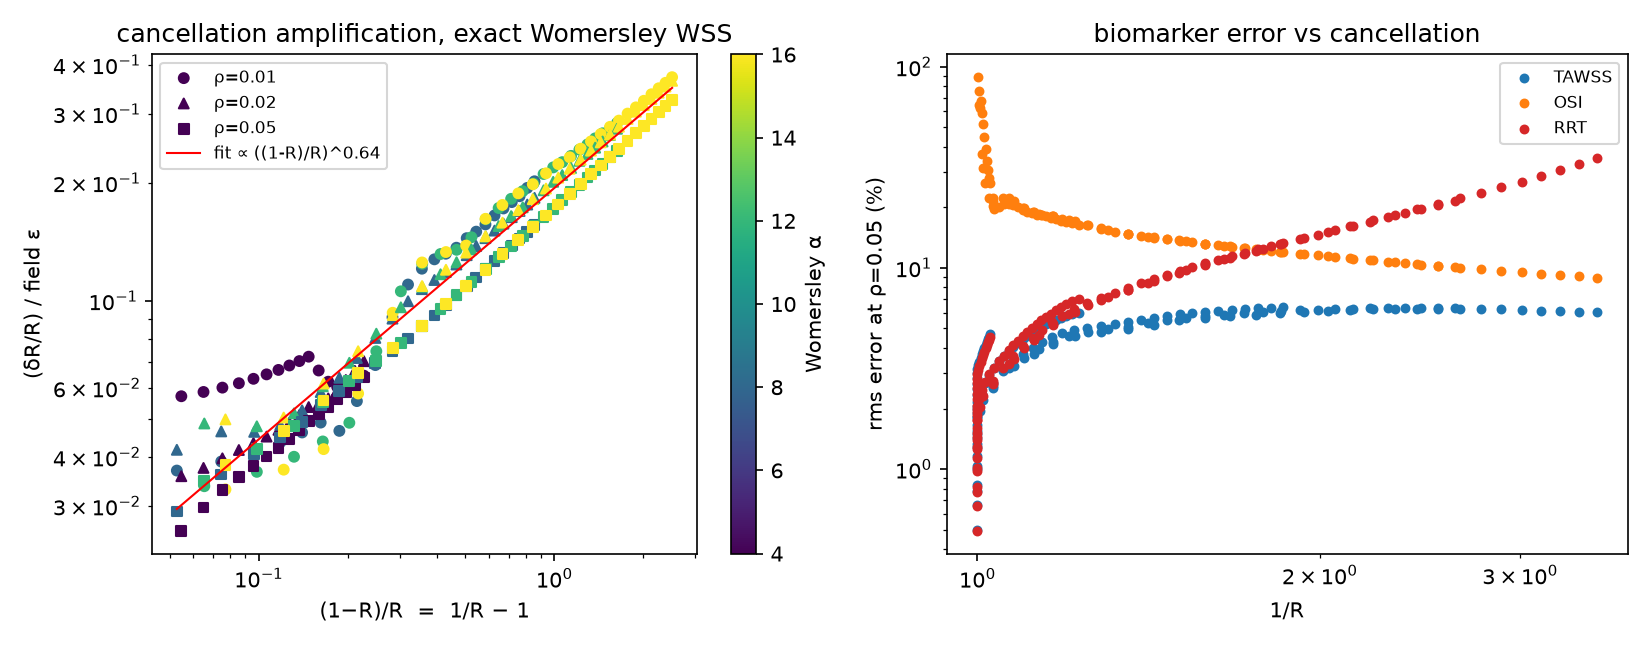
\includegraphics[width=0.85\textwidth]{figs/womersley_sweep.png}
\caption{Womersley sweep, $294$ reversing cases. Relative error of the
cancellation ratio per unit field error against the cancellation factor
$X=1/R-1$, with the fitted power law. The fitted exponent $0.64$ is explained
in Section~\ref{sec:window} as the $5/6$--$1$ crossover of \eqref{eq:window}
combined with the growth of $\eps/\rho$ with reversal; against $\rho$ the
exponent is $0.76$.}
\label{fig:womersley}
\end{figure}

\subsection{Validity of the first-order bias formula}
\label{sec:validity}

Because surrogate field errors are of order $10\%$ rather than infinitesimal,
the range of validity of \eqref{eq:bias} was mapped directly. The
three-dimensional form was evaluated per face on the cerebral CFD of
Section~\ref{sec:cfd} and compared with a measured isotropic frozen bias at
four amplitudes, averaged over four random directions
(\texttt{law\_theory\_bias.py}, \texttt{referee\_checks.py}).
Table~\ref{tab:validity} gives the ratio of predicted to measured median
$\delta R/R$.

\begin{table}[t]
\centering
\caption{Predicted over measured median $\delta R/R$ for a frozen isotropic
bias of relative magnitude $\eps$, cerebral wall, by cancellation-factor bin.
Face counts: $1797$, $281$, $86$, $9$.}
\label{tab:validity}
\begin{tabular}{l r r r r}
\toprule
$\eps$ & $X\in[0.02,0.1)$ & $[0.1,0.3)$ & $[0.3,1)$ & $[1,10)$\\
\midrule
$2\%$    & 1.11 & 1.02 & 1.04 & 1.33\\
$5\%$    & 1.09 & 1.03 & 1.06 & 1.31\\
$10.8\%$ & 1.07 & 1.05 & 1.05 & 1.31\\
$20\%$   & 0.96 & 1.07 & 1.11 & 1.22\\
\bottomrule
\end{tabular}
\end{table}

The formula is accurate to $11\%$ over $0.02\le X<1$ for field errors from
$2\%$ to $20\%$, so first order is an adequate description across the whole
range of surrogate accuracy currently reported. In the top bin it
over-predicts by about $30\%$. That discrepancy is \emph{independent of}
$\eps$, which rules out neglected higher-order terms as the cause; with only
$9$ contributing faces we regard it as a sampling effect and do not interpret
it further. Below $X=0.02$ the response is dominated by the second term of
\eqref{eq:master} and the prediction degrades to a factor of two; the formula
should not be used there, which is also the regime in which $\RRT$ is well
conditioned and the question does not arise.

\subsection{Why $\OSI$ appears fragile in a norm}

From \eqref{eq:chain}, $\delta\OSI/\OSI=-(R/(1-R))\,\delta R/R$, which grows
as $\OSI\to0$: per face, the relative error of $\OSI$ is worst exactly where
$\OSI$ is smallest. In an $L_2$ norm over a wall, however, the faces with
large $\OSI$ dominate the denominator, and on those faces the same expression
is small. The norm-level $\OSI$ error is therefore not a property of $\OSI$
but of the perturbation: white noise inflates it enormously, a window
mismatch barely at all. The frequently quoted statement that ``$\OSI$ blows
up because it is small'' is a per-face statement; the large $\OSI$ norm
errors reported in the surrogate literature are set by the error type, which
Section~\ref{sec:fingerprint} turns into a diagnostic.

\section{Patient-specific CFD}
\label{sec:cfd}

\subsection{Cases and numerical setup}

Two rigid-wall simulations were run with OpenFOAM v2512 (\texttt{pimpleFoam},
laminar, Newtonian blood with $\rho=\SI{1060}{kg/m^3}$ and
$\mu=\SI{3.5}{mPa.s}$; \texttt{backward} time scheme,
\texttt{linearUpwindV} convection, two PISO correctors and one
non-orthogonal corrector, fixed time step $\SI{1e-4}{s}$).

The cerebral case is a middle cerebral artery bifurcation aneurysm
($573\,297$ cells, $33\,406$ wall faces) segmented from anonymised DICOM data
distributed to participants of the International Aneurysm CFD Challenge
2015, Phase~I. The inlet uses a $40$-point tabulated volumetric flow rate of
period $T=\SI{0.9}{s}$ (peak $\SI{5.59}{mL/s}$ at phase $0.225$, diastole
decaying $33\%$ with no plateau) applied through
\texttt{flowRateInletVelocity}; the two outlets use \texttt{inletOutlet}
velocity with fixed zero gauge pressure, and the wall is no-slip. Three
cycles were run to $t=\SI{2.7}{s}$ with fields written every
$\SI{0.0225}{s}$, giving $40$ snapshots per cycle; the cycle-2 to cycle-3
difference is $1.2\times10^{-5}$ and cycle~3 is used throughout. The mean
Womersley number is $\alpha\approx2.2$. Inflow never reverses: only $0.34\%$
of the wall has $\OSI>0.1$ and the sac maximum is $0.085$; area-averaged
$\TAWSS=\SI{5.73}{Pa}$ and $\OSI=0.0032$. This case is therefore a
low-reversal control.

The abdominal aortic case is AAA042 from the Vascular Model Repository
($48\,345$ wall faces). Flow reversal is physiological here, but an outlet
backflow instability at reversal required a \texttt{totalPressure} outlet
condition, and the solution is only weakly periodic: seventeen cycles were
needed to reach a cycle-to-cycle difference of $2.66\%$, and cycle~17 is
used. Sac peak $\OSI$ is $0.209$, $2.5$ times the cerebral sac maximum.
Whole-wall averages are not comparable between the two geometries --- more
than $95\%$ of the AAA042 wall is non-reversing aorta and iliac, which
dilutes the average below the cerebral one --- so sac-to-sac comparison is
used throughout.

\subsection{Controlled perturbations}

The converged cycle is perturbed in four ways at matched offset-removed field
error: a period change integrated over the surrogate's own window; a window
mismatch (the period stretched by $1+\rho$ and the field re-interpolated onto
the patient's time grid, Section~\ref{sec:window}); a frozen isotropic
per-face bias (Section~\ref{sec:bias}); and temporally white noise
(Section~\ref{sec:noise}). Biomarkers are recomputed and compared to the
unperturbed cycle.

\begin{table}[t]
\centering
\caption{Cerebral wall, matched field error $\eps=10.8\%$: median per-face
$|\delta R/R|$ in \%, measured against the closed forms of
Sections~\ref{sec:window} and \ref{sec:bias}. Both measured and predicted
entries are the same quantity, so the comparison is like for like. Bias and
noise entries are rms over six random realisations.}
\label{tab:etype}
\begin{tabular}{l r r r r r}
\toprule
& $X\in[0,0.02)$ & $[0.02,0.1)$ & $[0.1,0.3)$ & $[0.3,1)$ & $[1,10)$\\
\midrule
faces & 31\,233 & 1797 & 281 & 86 & 9\\
\midrule
period change, own window & 0.000 & 0.000 & 0.000 & 0.000 & 0.000\\
window mismatch, $\rho=5\%$ & 0.001 & 0.060 & 0.252 & 1.509 & 3.669\\
\quad predicted, \eqref{eq:window} & 0.000 & 0.000 & 0.000 & 2.367 & 4.378\\
frozen bias & 0.365 & 1.617 & 2.521 & 6.175 & 16.618\\
\quad predicted, \eqref{eq:bias} & 0.197 & 1.582 & 2.698 & 6.256 & 19.232\\
white noise & 0.879 & 1.425 & 1.038 & 1.240 & 3.338\\
\bottomrule
\end{tabular}
\end{table}

Table~\ref{tab:etype} tests the two closed forms directly and recovers the
predicted ordering. A period change integrated over the surrogate's own
period costs nothing, exactly. At matched field error a frozen bias costs
four to five times more than a window mismatch in every reversing bin, as the
larger prefactor of \eqref{eq:bias1d} requires, and white noise costs least
where cancellation is strong.

The three-dimensional bias formula \eqref{eq:bias} predicts the measured
response closely: $1.58$ against $1.62$, $2.70$ against $2.52$, $6.26$
against $6.18$ and $19.2$ against $16.6$ per cent in the four reversing bins,
i.e.\ within $16\%$ throughout. Below $X=0.02$ it under-predicts by a factor
of two, as Section~\ref{sec:validity} documents.

The window-mismatch formula \eqref{eq:window}, by contrast, agrees only in
the two most reversing bins ($2.37$ against $1.51$ and $4.38$ against $3.67$)
and returns exactly zero in the middle bins where the measured response is
small but non-zero. The reason is instructive and is a genuine limitation of
that result: \eqref{eq:window} is a one-dimensional relation, derived for a
shear that reverses along a fixed direction, and applied per face we evaluate
it on the component of $\boldsymbol\tau$ along $\hat{\mathbf s}$. Where the
cancellation is transverse rather than antiparallel --- the parallel
component never changing sign while the direction of $\boldsymbol\tau$
swings --- that component has $m_-=0$ and the formula returns zero, whereas
the true response is finite. Equation~\eqref{eq:window} should therefore be
read as exact for unidirectional reversing flow, which is the Womersley case
of Section~\ref{sec:sweep} and the regime it was derived for, and as a lower
bound per face in three dimensions. The bias relation \eqref{eq:bias} carries
no such restriction because it is vectorial from the outset.

On the whole wall at $\rho=5\%$ the raw field $L_2$ is $10.8\%$ while
$\TAWSS/\RRT$ errors are $2.47/2.54\%$ (wall), $3.44/3.57\%$ (sac, $784$
faces) and $1.51/2.42\%$ on the $\OSI>0.1$ faces ($115$) --- $\RRT$ amplified
$1.6$ times only where cancellation is present.

On AAA042 (Figure~\ref{fig:aaa}) the $\RRT$ amplification
$(\delta\RRT/\RRT)/(\delta\TAWSS/\TAWSS)$ against $\OSI$ has a log--log slope
of $+0.49$, in the cancellation-favouring direction. We attach no
quantitative weight to this figure: the $2.66\%$ periodicity floor exceeds
the smallest injected perturbations, and only the sign and rough magnitude of
the trend are meaningful. AAA042 is retained because its sac reaches
$\OSI=0.209$, but it contributes no faces above $X=1$ and only sixteen above
$X=0.1$.

\begin{figure}[t]
\centering
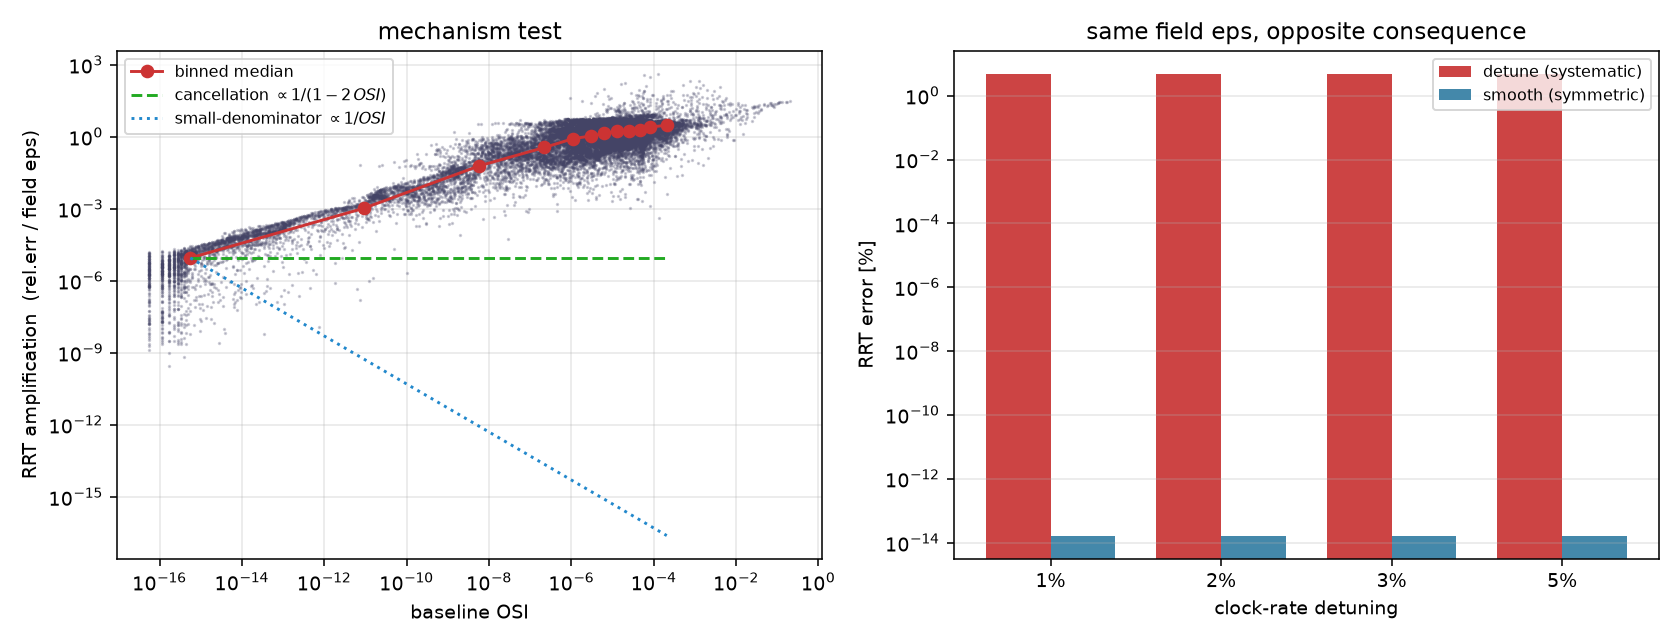
\includegraphics[width=0.85\textwidth]{figs/mechanism_test_aaa042_v2.png}
\caption{AAA042: per-face $\RRT$ amplification versus $\OSI$ under an
injected window mismatch on the periodic cycle. Trend only; see text.}
\label{fig:aaa}
\end{figure}

\section{A trained surrogate: POD\,+\,LSTM at an unseen heart rate}
\label{sec:lstm}

\paragraph{Model and training.}
Ten POD modes capture $99.998\%$ of the WSS energy on the cerebral wall; the
compressor alone gives $0.25\%$ field error and $\approx0\%$ $\RRT$ error, so
it is not the bottleneck. An LSTM is trained on latent trajectories of beats
with $34$--$46$ samples per period and tested by autoregressive rollout on
the unseen $40$-sample beat against the CFD truth. A model trained and tested
on the same beat memorises it with zero drift and is kept as a baseline.

\paragraph{Validity of the heart-rate augmentation.}
Beats at other heart rates are generated by time-stretching, which is an
approximation: the Womersley number varies as $f^{1/2}$, so the range used
corresponds to $58$--$\SI{78}{bpm}$ and $\alpha=2.03$--$2.37$, a $\pm8\%$
excursion about the baseline $2.18$. To bound the resulting error, the exact
Womersley solution was evaluated for the measured inlet waveform at
$T=0.765$, $0.900$ and $\SI{1.035}{s}$ and each compared with the
time-stretch of the baseline. The true and stretched wall shear differ by
$2.7\%$ and $2.2\%$ in field $L_2$ respectively, and the cycle-averaged
biomarkers are unchanged to machine precision because this waveform does not
reverse. The augmentation therefore introduces a shape error an order of
magnitude smaller than the rollout errors under study, but it is not a
substitute for simulating each heart rate, and on a reversing geometry the
biomarker invariance would not hold.

\paragraph{What the usual metric says, and what the rollout does.}
Teacher-forced one-step RMSE on the unseen beat is $7.3\times10^{-2}$ in
latent units --- the number a paper would normally report. Over six beats the
raw field $L_2$ grows from $7.8\%$ to $79\%$; after removing the best global
offset it stays between $2\%$ and $10\%$, and the lag grows by about $0.7$
samples per beat. A $40$-beat rollout is a clean limit cycle with spectral
peaks at $1.013$, $2.026$, $3.038$ and $4.051$ per beat, i.e.\ a clock
$1.3\%$ fast, plus a weak $\approx18$-beat modulation (sidebands at $+0.055$
per beat on mode~2). On the $\OSI>0.1$ faces the $\RRT$ error is $2.3$ to
$2.7$ times the $\TAWSS$ error (Table~\ref{tab:lstm}), consistent with
\eqref{eq:chain}.

\begin{table}[t]
\centering
\caption{POD\,+\,LSTM rollout on the unseen beat. Errors in \%; T/R denotes
$\TAWSS$/$\RRT$. Region sizes: wall $33\,406$ faces, sac $784$,
$\OSI>0.1$ $115$.}
\label{tab:lstm}
\begin{tabular}{r r r c c c}
\toprule
beat & raw $L_2$ & lag (samples) & wall T/R & sac T/R & $\OSI>0.1$ T/R\\
\midrule
1 & 7.8 & 0.0 & 6.23/6.78 & 8.84/10.24 & 3.00/6.94\\
2 & 31.2 & $-1.0$ & 7.72/8.59 & 11.59/13.93 & 3.78/9.40\\
3 & 63.1 & $-2.6$ & 2.19/2.30 & 1.99/2.30 & 1.22/1.17\\
4 & 55.6 & $-2.1$ & 9.16/10.40 & 13.36/16.64 & 4.33/11.00\\
5 & 77.3 & $-3.8$ & 1.90/1.88 & 2.62/2.62 & 0.85/1.91\\
6 & 78.9 & $-4.0$ & 1.50/1.56 & 3.54/3.77 & 1.50/4.11\\
\bottomrule
\end{tabular}
\end{table}

\paragraph{Truth-free clock diagnosis.}
Treating the rollout as a limit cycle, the rate error is estimated from the
rollout alone by fitting a single frequency scaling to its own phase, a
phase-reduction view following the treatment of bluff-body wakes
in~\cite{samanta2026}. On six beats it returns $+1.66\%$ against a
ground-truth lag growth of $+1.98\%$; on $40$ beats it returns $+1.41\%$, in
agreement with the spectral estimate. After re-timing, the residual
self-rate is $-0.03\%$ and the lag stays bounded within $[-2.6,0]$ samples
over $40$ beats, where the raw lag reached $-20$ samples and wrapped
(Figure~\ref{fig:phase}). On a synthetic rollout with a known $2\%$ drift the
estimate returns $1.99\%$ and re-timing reduces $\RRT$ error by a factor
of~$30$.

\paragraph{Re-timing does not repair the biomarkers, and the theory says why.}
On the real rollout, mean $\RRT$ error after the transient moves only from
$4.95$ to $4.54\%$ (wall), $7.85$ to $7.09\%$ (sac) and $5.52$ to $5.10\%$
($\OSI>0.1$). A perfect-shape model with a $1.5\%$ clock error would give
about $0.8\%$ $\RRT$ error, so roughly $80\%$ of the error is beat shape and
the slow modulation; $\RRT$ error tracks the offset-removed $L_2$, not the
lag. The diagnosis is therefore ``re-timing will not help; improve the
model'', and it is available without ground truth.

The residual is also quantitatively consistent with the theory, in an
instructive way. Applying the window-mismatch formula \eqref{eq:window} with
the offset-removed $\eps=3.7\%$ predicts $0.8\%$ excess $\RRT$ error in the
top cancellation bin, against $7.0\%$ measured --- low by a factor of nine.
But after re-timing the residual is by construction no longer a window
mismatch: it is beat-shape error, persistent across the rollout and therefore
closer to the bias case of Section~\ref{sec:bias}, whose exponent is $1$
rather than $0.76$ and whose prefactor is about five times larger. The
under-prediction is the expected signature of applying the wrong error model,
and is itself part of the diagnosis.

\begin{figure}[t]
\centering
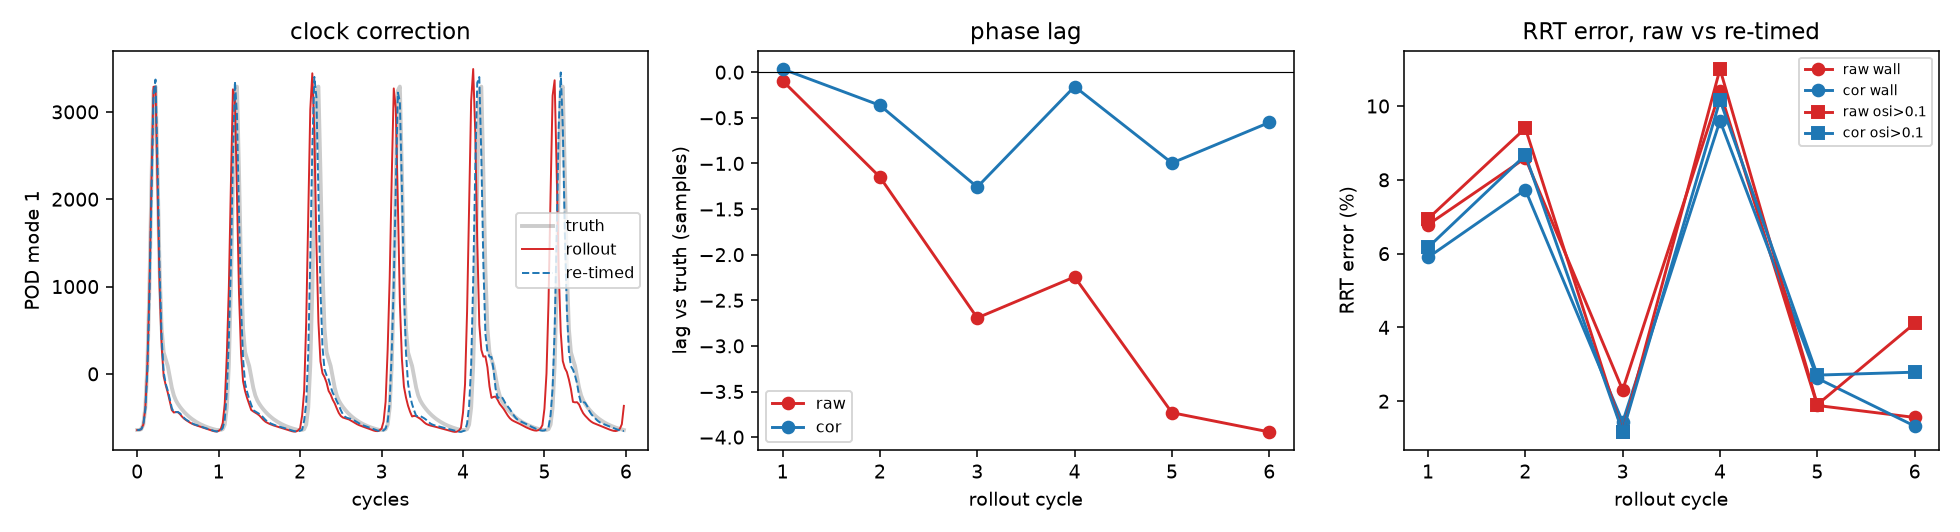
\includegraphics[width=0.85\textwidth]{figs/phase_correct_hr.png}
\caption{Truth-free clock estimate and re-timing on the six-beat rollout.}
\label{fig:phase}
\end{figure}

\section{The error triple as a fingerprint}
\label{sec:fingerprint}

\subsection{Separation by error type}

The cerebral cycle was perturbed by the three error types at matched field
error and scored with the mean-based relative $L_2$ used
by~\cite{rhsia2026}, $\|X_{\rm pred}-X_{\rm true}\|_2/\|X_{\rm true}\|_2$
over faces, so that the numbers are directly comparable with that paper's
Table~V. Results are in Table~\ref{tab:fp}.

\begin{table}[t]
\centering
\caption{Biomarker error ratios by error type on the cerebral wall,
mean-based $rL_2$ in \%, beside the published values of~\cite{rhsia2026},
obtained on a per-snapshot graph model over intracranial aneurysm surfaces.
Frozen-bias entries vary by $\pm15\%$ with the random seed.
$^{\dagger}$this row propagates \eqref{eq:window} face by face under the
assumption $\delta\TAWSS/\TAWSS=\eps$, and is shown to make the point that a
window-mismatch model cannot reproduce the published ratios.}
\label{tab:fp}
\begin{tabular}{l r r r r r r}
\toprule
perturbation & $\eps$ & $\TAWSS$ & $\OSI$ & $\RRT$ & $\OSI/\TAWSS$ & $\RRT/\TAWSS$\\
\midrule
\eqref{eq:window} applied per face$^{\dagger}$ & 13.5 & 13.5 & 5.1 & 13.6 & 0.37 & 1.00\\
window mismatch $\rho=5\%$ & 10.8 & 2.5 & 3.1 & 3.5 & 1.22 & 1.37\\
white noise & 13.5 & 2.3 & 68.7 & 2.5 & 30 & 1.08\\
frozen bias & 13.5--16 & 10--12 & 57--75 & 14--19 & 5.6--6.3 & 1.4--1.6\\
\midrule
published~\cite{rhsia2026} & -- & 13.54 & 68.35 & 17.31 & 5.05 & 1.28\\
\bottomrule
\end{tabular}
\end{table}

Two things follow. First, $\RRT/\TAWSS\approx1.3$ is obtained for every error
type on a weakly reversing wall and matches the published $1.28$: on such a
wall \eqref{eq:chain} reduces to $\delta\RRT\approx\delta\TAWSS$ plus a small
cancellation term, and an independently trained model on different geometries
confirms it. Second, $\OSI/\TAWSS$ separates the error types by more than an
order of magnitude, and only a time-coherent per-node bias reproduces the
published $5.05$. That is the error one expects from a model regressing each
snapshot independently from geometry, the case of Section~\ref{sec:bias}: its
mistakes are spatial and persistent, not temporal. The window-mismatch
formula predicts $0.37$ and is simply the wrong error model for that
surrogate, which the fingerprint detects without being told. The
corresponding author of~\cite{rhsia2026} confirms the reading: ``you were
right about the RRT error of my surrogate model, they present spatial error
and usually persistent'' (W.~Ding, personal communication, 2026).

\subsection{The bands depend on the wall's $\OSI$ distribution}
\label{sec:bands}

The separation in Table~\ref{tab:fp} is computed on one wall and must not be
treated as a set of universal thresholds. To quantify the dependence, the
same three perturbations were scored on nested subsets of the cerebral wall
of progressively higher $\OSI$ (Table~\ref{tab:bands}).

\begin{table}[t]
\centering
\caption{$\OSI/\TAWSS$ error ratio by error type, on nested subsets of the
cerebral wall of increasing median $\OSI$.}
\label{tab:bands}
\begin{tabular}{l r r r r r}
\toprule
face subset & faces & median $\OSI$ & window mismatch & white noise & frozen bias\\
\midrule
whole wall    & 33\,406 & 0.0007 & 1.22 & 27.4 & 4.78\\
$\OSI>0.002$  & 7234    & 0.0048 & 1.13 & 16.5 & 3.94\\
$\OSI>0.01$   & 2146    & 0.0212 & 1.14 & 10.5 & 3.56\\
$\OSI>0.03$   & 635     & 0.0503 & 1.27 & 5.00 & 2.25\\
\bottomrule
\end{tabular}
\end{table}

The window-mismatch band is stable at $1.1$--$1.3$, but the noise and bias
bands fall by factors of five and two as the wall's median $\OSI$ rises by
two orders of magnitude, and on the most strongly reversing subset the three
types are separated by less than a factor of four. The diagnostic is
therefore reliable on walls whose $\OSI$ distribution is dominated by small
values --- the case for the intracranial surfaces of most published
surrogates, and stated explicitly in~\cite{rhsia2026} --- and it should be
recalibrated on the geometry at hand rather than read off Table~\ref{tab:fp}.
The comparison with~\cite{rhsia2026} above uses the whole-wall row, matching
their stated $\OSI$ distribution; that match is an assumption, since their
fields are not public.

With that caveat, the practical rule is: a ratio near unity with a drifting
lag indicates a window mismatch, and re-timing is the remedy; a very large
ratio with small $\TAWSS$ and $\RRT$ errors indicates temporal noise, which
smoothing removes without touching $\RRT$; an intermediate ratio with
comparable $\TAWSS$ and $\RRT$ errors indicates persistent spatial bias,
which only a better model repairs.

\section{Discussion}

\paragraph{What is new.}
The master relation \eqref{eq:master} is elementary, and we make no claim
otherwise. Its value is in the consequences, which are routinely violated in
current practice: scoring a rollout by raw $L_2$ when a time shift is
biomarker-neutral; reading a large $\OSI$ error as a property of $\OSI$
rather than of the perturbation; reporting one-step accuracy for a model
whose limit cycle runs at the wrong rate; and transferring one error type's
constants to a different error type. To our knowledge the closed forms
\eqref{eq:window} and \eqref{eq:bias}, the exact smoothing invariance of
$\RRT$, and the use of the reported error triple as an error-type diagnostic
have not appeared previously.

\paragraph{Relation to residence time as a biomarker.}
It has been argued that $\RRT$ is at best an imperfect proxy for Lagrangian
residence time. That question is orthogonal to the present one. We analyse
the conditioning of $\RRT$ as it is defined and reported, not its biological
validity: even a surrogate that reproduced the WSS field well would
mis-estimate $\RRT$ wherever cancellation is strong, and a reader who prefers
a Lagrangian measure still needs to know that the shear-based proxy they
compare against is ill-conditioned in exactly the regions of interest.

\paragraph{Clinical relevance and its limits.}
The motivation for these biomarkers is rupture and thrombosis risk
stratification, and the natural question is whether the errors described here
are large enough to change a classification. We cannot answer that from the
present data: it would require a cohort, an accepted $\RRT$ threshold and a
labelled outcome, none of which are available here. What can be said is that
the errors are concentrated, by construction, in the low-shear reversing
regions that such thresholds are designed to detect, so error and signal are
co-located rather than independent. Establishing the resulting
misclassification rate on a labelled cohort is the natural next step and the
one we would prioritise.

\paragraph{Limitations.}
\begin{itemize}
\item The closed forms are first order in $|\mathbf d|/|\boldsymbol\tau|$ and
assume the perturbation does not itself alter the sign structure of the
waveform. Section~\ref{sec:validity} maps the resulting accuracy: better than
$11\%$ for $0.02\le X<1$ and $\eps\le20\%$, degrading to a factor of two
below $X=0.02$.
\item Both patient geometries are weakly reversing. The cerebral wall
contributes $9$ faces above $X=1$ and AAA042 none; the strong-cancellation
regime rests on the analysis and on the Womersley sweep. A reversing patient
geometry --- infrarenal aorta, left atrial appendage or a fusiform aneurysm
--- is the most valuable single addition to this work.
\item AAA042 reaches only a $2.66\%$ cycle-to-cycle floor, and its
mesh-independence was checked at a non-periodic state; its numbers are
reported as trends only.
\item The fingerprint bands depend on the wall's $\OSI$ distribution
(Section~\ref{sec:bands}), and real surrogate errors are mixtures of the
three types. The diagnostic identifies the dominant type; it does not
decompose a mixture, and we have not established the mixing fraction at which
it fails.
\item The external validation uses published aggregate numbers, not the
model's fields. A per-node test on a released model would be a considerably
stronger check.
\item Equation~\eqref{eq:window} is one-dimensional. Applied per face in
three dimensions it is a lower bound, exact where reversal is antiparallel
and vanishing where cancellation is purely transverse
(Section~\ref{sec:cfd}); a vectorial generalisation is left open. The bias
relation \eqref{eq:bias} has no such restriction.
\item The $5/6$ exponent requires a non-degenerate zero crossing
(Section~\ref{sec:window}), and a single surrogate architecture was trained
here.
\end{itemize}

\section*{Data, code and ethics}

The cerebral geometry was segmented from anonymised images distributed for
the 2015 International Aneurysm CFD Challenge~\cite{challenge2018}, which
comprised five middle cerebral artery aneurysms. Institutional review board
approval for sharing those anonymised images was obtained by the challenge
organisers from Wakayama Rosai Hospital, as reported
in~\cite{challenge2018}; no new patient data were collected and no
identifiable information was accessed for the present study, which is a
secondary computational analysis. AAA042 is a public case from the Vascular
Model Repository. All analysis
scripts (\texttt{womersley\_sweep.py}, \texttt{law\_theory.py},
\texttt{law\_theory\_bias.py}, \texttt{law\_vs\_errortype.py},
\texttt{referee\_checks.py}, \texttt{pod\_lstm\_hr\_v2.py},
\texttt{phase\_correct\_v2.py}, \texttt{mechanism\_test\_aaa042\_v2.py},
\texttt{rhsia\_check\_v[1-3].py}) and the reduced data needed to reproduce
every figure and table are available at
\url{https://github.com/Syphonicc/shear-drift}, with an interactive version
of the analysis at \url{https://syphonicc.github.io/shear-drift/}.

\section*{Funding and competing interests}

This research received no external funding. The author declares no competing
interests.

\section*{Acknowledgements}

The author thanks Sachidananda Behera for discussions, and Wenhao Ding
(Imperial College London) for the observation that a period change integrated
over the surrogate's own cycle leaves the biomarkers unchanged, which
corrected Section~\ref{sec:window}, and for permission to quote his
assessment in Section~\ref{sec:fingerprint}.

\begin{thebibliography}{9}
\bibitem{npj2026} Physics-constrained graph neural network for real-time
prediction of intracranial aneurysm hemodynamics. \emph{npj Digital Medicine}
(2026). \url{https://doi.org/10.1038/s41746-026-02404-z}
\bibitem{jekenrico2025} Graph deep learning for intracranial aneurysm blood
flow simulation and risk assessment. arXiv:2512.09013 (2025).
\bibitem{rhsia2026} Real-time pulsatile flow prediction for realistic,
diverse intracranial aneurysm morphologies using a graph transformer and
steady-flow data augmentation. arXiv:2601.19876v2 (2026).
\bibitem{rygiel2025} Rapid wall shear stress prediction for aortic aneurysms
using deep learning. \emph{Med.\ Biol.\ Eng.\ Comput.} (2025).
\url{https://doi.org/10.1007/s11517-025-03311-3}
\bibitem{aaa2025} Wall shear stress estimation in abdominal aortic aneurysms:
towards generalisable neural surrogate models. arXiv:2507.22817 (2025).
\bibitem{sarrami2016} Sarrami-Foroushani A.\ et al. Uncertainty
quantification of wall shear stress in intracranial aneurysms using a
data-driven statistical model of systemic blood flow variability.
\emph{J.\ Biomech.} 49 (2016).
\bibitem{bergersen2017} Bergersen A.\ W.\ et al. Robustness of common
hemodynamic indicators with respect to numerical resolution in 38 middle
cerebral artery aneurysms. \emph{PLoS ONE} 12 (2017) e0177566.
\bibitem{mri2016} Cibis M.\ et al. The effect of spatial and temporal
resolution of cine phase-contrast MRI on wall shear stress and oscillatory
shear index assessment. \emph{PLoS ONE} 11 (2016) e0163316.
\bibitem{challenge2018} Valen-Sendstad K.\ et al. Real-world variability in
the prediction of intracranial aneurysm wall shear stress: the 2015
International Aneurysm CFD Challenge. \emph{Cardiovasc.\ Eng.\ Technol.} 9
(2018) 544--564. Data: \url{https://doi.org/10.6084/m9.figshare.6383516}
\bibitem{samanta2026} Samanta S., Behera S. Autoregressive rollout error in
latent-space reduced-order models of bluff-body wakes is accumulated phase
drift. arXiv:2608.07189 (2026).
\end{thebibliography}

\end{document}
